\chapter{Implementation}
\label{chapter-6}

This chapter primarily discusses the steps and modifications that has been carried out to tune the software. The imitation 
is performed initially with upper body and then to lower body eventually testing the complex motions considering the NAO robot's 
structure. The results of the implementation will be discussed in the coming sections later in this chapter.


\section{Methodology}

The implementation began by testing the robot's kinematics already implemented in order to obtain relation between it's joints  and task spaces.
Once the suitable implementation has been validated, the captured human data is scaled down to the robot's size and it's desired parameters $\Omega$
are retrieved for HQP.

\begin{figure}[h!]
    \centering
    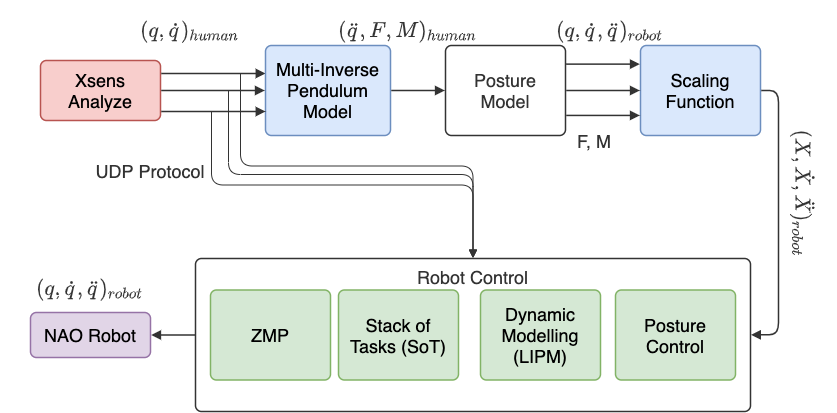
\includegraphics[scale=0.5]{images/flowchart-block-diagram.png}\hfill
    \caption{Block Diagram Representation of Imitation Program}\hfill
    \label{fig: block-diagram}
\end{figure}

Figure \ref{fig: block-diagram} represents the flow of data between individual blocks discussed in chapter \ref{chapter-3} and 
chapter \ref{chapter-4}. It is notable that two computers are used for this implementation to extract convenient results.

\section{Robot Model}

During the course of this research, both real robot and virtual models are used. The real robot used for validation is
a NAO v5 H25 Humanoid robot and the virtual model is a CopelliaSim model with approximately equivalent inertial modelling.
Like previous implementations on kinematic modelling \cite{louisepouble}, the hand operations (open/close) will be ignored therby
controlling 23 DoFs in total (vector $q$). Figure \ref{fig: nao-robot-joint} represents the arrangement of DoFs that will be used in this research.

\begin{equation*}
    q = \begin{bmatrix}
        q_1 && q_2 && ... & q_{23}
    \end{bmatrix}^T
\end{equation*}
\begin{figure}[h!]
    \centering
    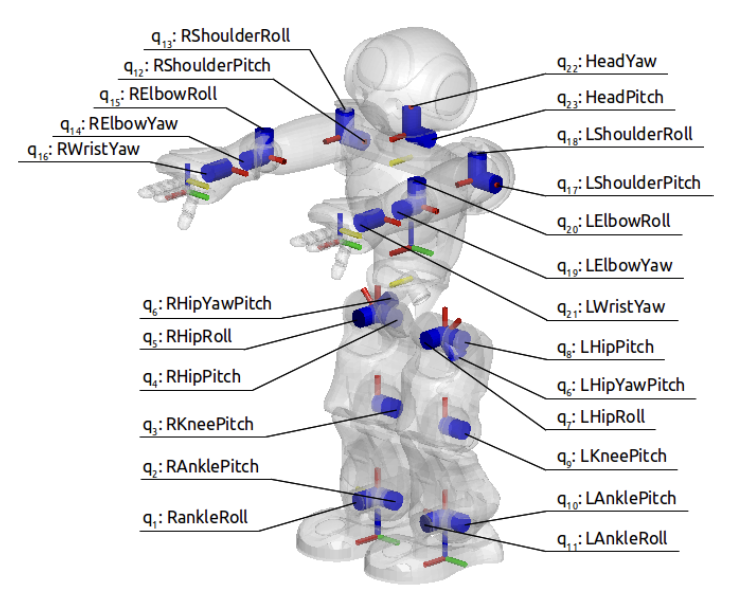
\includegraphics[scale=0.55]{images/nao-robot-joint.png}\hfill
    \caption{NAO Robot's DoF Arrangement \cite{louisepouble}}\hfill
    \label{fig: nao-robot-joint}
\end{figure}

\subsection{Kinematic Modelling}

The robot's geometric model was calculated using the nominal approach with \textit{Modified Denavit-Hartenberg} (MDH) parameters. Since the 
robot is a tree structure, some links have more than one child links. In addition, it might be convenient to include 
frames in the model which are not necessarily defined according to the previous rules. Then, the kinematic model can be represented as,

\begin{equation}
    \label{eq: robot-dgm-1}
    \begin{bmatrix}
        \dot{x}_{lhand} \\ \dot{x}_{rhand} \\ \dot{x}_{lleg} 
    \end{bmatrix} = J \begin{bmatrix}
        \dot{q}_{lhand} \\ \dot{q}_{rhand} \\ \dot{q}_{lleg}
    \end{bmatrix}
\end{equation}

Equation \ref{eq: robot-dgm-1} can be simply represented as $\dot{X} = J\dot{q}$ in the next sections where $J$ is the robot Jacobian and $x_i$ is a $3 \times 1$ vector without
considering the end-effector oriendation. The above equation has a vector size of $(6 + 6 +5) \times 1$ considering only three kinematic chains for the sake of redundancy. 
In other words, the right foot will always be in contact with the floor. 
This work was implemented in MATLAB and was exported to a C++ library "Jacobian" (available in \cite{github}). 

\subsection{Masses and CoM}

The robot's dynamic parameters like masses and Centre of Masses can be obtained from the 
documentation directly \cite{aldebaran-masses}. The individual masses and CoM for each link 
is calculated and documented in the website. To calculate the single point mass and the projection of 
CoM onto xy plane is,

\begin{align}
    \label{eq: robot-mass-com}
    M &= \Sigma_{i = 1}^n m_i \\
    P_{CoM} &= \frac{1}{M}\Sigma_{i = 1}^n m_ic_i
\end{align}

where $m_i$ and $c_i$ represent the individual mass and CoM of link $i$ obtained from documentation respectively; n is the number of moving masses 
in the robot body. The jacobian of CoM can then be formulated with respect to the robot frame (frame located at right foot) is given by,

\begin{align}
    \label{eq: robot-mass-com-2}
    J_{CoM} &= \frac{\partial P_{CoM}}{\partial q} \quad \mathit{or} \\
    \dot{P}_{CoM} &= J_{CoM} \dot{q}
\end{align}

The size of $J_{CoM}$ is $2 \times 23$ (reflection of CoM onto 2D plane (x, y)). $P_{CoM}$ is a 2-dimensional vector since the projection on xy plane.

\section{Human Motion}

The sensor data acquired from Xsens suit is high-quality less-noise data with the ability to record wide range of motions.
The data acquired greatly differ in cartesian sizing compared to the size of the NAO robot. Usually in motion imitation, the robot 
must reach the same point in task space as the human actor, but due to greater difference in size, the task space is treated as relative instead of absolute. 
To achieve this criteria, a scaling function need to be implemented before
feeding the Xsens data to the robot control.

\subsection{Scaling Function}

In a previous work \cite{scaling-human-nao}, the use of a scaling factor for each limb based on the ratio between the lengths of the kinematic chain of actor and 
imitator was proposed. This factor was then multiplied by the captured human data to obtain the desired positions for the robot. Since each limb 
was a simple serial chain, a proportional scaling factor could be applied satisfactorily.

However, in the present work, the balance is being taken into account and thus the robot has to be modelled as a whole, which gives rise to s 
tree-structure. In this case, keeping the direction of the captured human data means that the robot’s end-effectors will fall on the line which 
connects the tracked points to the origin on the right foot.

\begin{figure}[h!]
    \centering
    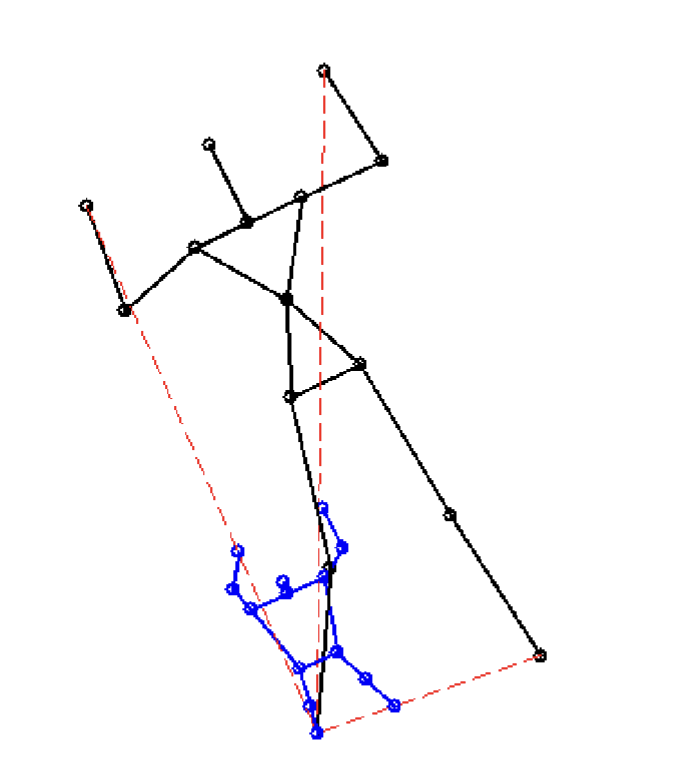
\includegraphics[scale=0.7]{images/proportional-scaling.png}\hfill
    \caption{Proportional scaling of human motion \cite{louisepouble}}\hfill
    \label{fig: proportional scaling}
\end{figure}

A new scaling method is proposed in \cite{sakka:hal-01054887} which takes into account not only the
lengths of each of the segments but also each of their directions. This way, the captured
human motion is scaled segment by segment to the lengths of the robot while keeping the 
direction of that segment. The iterative process starts from the right ankle and moves upwards towards each of the end-effectors.

In summary considering a link $l$, the scaling can be processed as,

\begin{equation}
    P_l^{robot} = \frac{P_l^{human} - P_a^{human}}{||P_l^{human} - P_a^{human}||}l_l^{robot} + P_a^{robot}
\end{equation}

~

where $P_a$ refers to the antecedent position to the link $l$. Since the robot doesn’t have a spine, the distances connecting shoulders and hips 
should remain constant. The shoulders cannot be scaled directly from the hips because of the different torso proportions between the human and the 
robot. It was chosen to scale a segment which goes from the point between the hips to the point between the shoulders, preserving symmetry.